% --------------------------------------------------------------
% This is all preamble stuff that you don't have to worry about.
% Head down to where it says "Start here"
% --------------------------------------------------------------
 
\documentclass[10pt]{article}
%\setlength\parindent{24pt}  ??????????

\usepackage[margin=0.8in]{geometry} 
\usepackage{amsmath,amsthm,amssymb}
\usepackage{setspace}
\usepackage{amssymb}
\usepackage{amsmath}
\usepackage{amsthm}
\usepackage{latexsym}
\usepackage{enumerate}
\usepackage{setspace}
\usepackage{mathrsfs}
\usepackage[colorlinks=true, urlcolor=blue]{hyperref} % This package enables hyperlinks
\renewcommand{\qedsymbol}{$\blacksquare$} %This command makes the end-of-proof boxes solid black.
\usepackage{amscd}
\usepackage{mathtools}
\usepackage{graphicx}

\usepackage{siunitx} % Required for alignment

\sisetup{
  round-mode          = places, % Rounds numbers
  round-precision     = 2, % to 2 places
}


\makeatletter
\renewcommand*\env@matrix[1][*\c@MaxMatrixCols c]{%controls position of matrix elements.
  \hskip -\arraycolsep
  \let\@ifnextchar\new@ifnextchar
  \array{#1}}
\makeatother
 
\newcommand{\N}{\mathbb{N}}
\newcommand{\Z}{\mathbb{Z}}
\def\ep{\varepsilon}
\def\bR{\mathbb{R}}
\def\S{\mathbb{S}}
\def\C{\mathbb{C}}
\def\CP{\mathbb{CP}}
\def\bA{\mathscr{A}}
\def\lA{\lambda}
\def\a{\alpha}
\def\g{\gamma}
\def\e{\epsilon}
\def\p{\partial}
\def\sB{\mathscr{B}}
\def\la{\langle}
\def\ra{\rangle}
\newcommand{\norm}[1]{\left\lVert#1\right\rVert}
\def\n{\norm}
\def\o{\overline}


\newmuskip\pFqskip % this code is for the Hypergeometric notation
\pFqskip=6mu
\mathchardef\pFcomma=\mathcode`, % keep a copy of the comma

\newcommand*\pQq[5]{%this code is a continuation of the Hypergeometric notation
  \begingroup
  \begingroup\lccode`~=`,
    \lowercase{\endgroup\def~}{\pFcomma\mkern\pFqskip}%
  \mathcode`,=\string"8000
  {}_{#1}\phi_{#2}\biggl(\genfrac..{0pt}{}{#3}{#4};#5\biggr)%
  \endgroup
}

\renewcommand{\labelitemi}{$\textendash$} %this code resets the top list marker to a dash

 
\newenvironment{theorem}[2][Theorem]{\begin{trivlist}
\item[\hskip \labelsep {\bfseries #1}\hskip \labelsep {\bfseries #2.}]}{\end{trivlist}}
\newenvironment{lemma}[2][Lemma]{\begin{trivlist}
\item[\hskip \labelsep {\bfseries #1}\hskip \labelsep {\bfseries #2.}]}{\end{trivlist}}
\newenvironment{exercise}[2][Exercise]{\begin{trivlist}
\item[\hskip \labelsep {\bfseries #1}\hskip \labelsep {\bfseries #2.}]}{\end{trivlist}}
\newenvironment{reflection}[2][Reflection]{\begin{trivlist}
\item[\hskip \labelsep {\bfseries #1}\hskip \labelsep {\bfseries #2.}]}{\end{trivlist}}
\newenvironment{proposition}[2][Proposition]{\begin{trivlist}
\item[\hskip \labelsep {\bfseries #1}\hskip \labelsep {\bfseries #2.}]}{\end{trivlist}}
\newenvironment{corollary}[2][Corollary]{\begin{trivlist}
\item[\hskip \labelsep {\bfseries #1}\hskip \labelsep {\bfseries #2.}]}{\end{trivlist}}


% For an exam, single spacing is most appropriate
%\singlespacing
% \onehalfspacing%%%
% \doublespacing

% For an exam, we generally want to turn off paragraph indentation
\parindent 0ex
%\def\baselinestretch{2} % double spacing

\begin{document}
%\doublespacing
 
% --------------------------------------------------------------
%                         Start here
% --------------------------------------------------------------
 
%\renewcommand{\qedsymbol}{\filledbox}
 
\title{Lake Michigan Influences}%replace X with the appropriate number
\author{Blake Wallace\\ %replace with your name
Capstone Technical Report} %if necessary, replace with your course title
\date{May 17, 2019}
 
\maketitle

\vspace{2mm}

\begin{enumerate}[\null]

\item \textbf{Data science objectives}:
\begin{enumerate}
\item[1.] Does Rain have any effect on the average daily temperatures?
\item[2.] What effect does rain have on the average daily temperature near the water?
\item[3.] What effect does rain have on the average daily temperature far from the water?
\item[4.] When it rains, is there a statistically significant difference between the amount of rain that falls in downtown Chicago compared to the Ohare airport?
\item[5.] How much correlation exists between the average daily temperature of Lake Michigan and the temperature difference between the downtown Chicago area and the Ohare airport?
\item[6.] Can we build a model that predicts with at least 80\% accuracy the difference in total precipitation between Ohare airport and the the Botanical gardens?
\item[7.] Is there a statistically significant difference between the daily temperature near the water as apposed to far from the water?
\end{enumerate}
 


\item \textbf{Data Sources}: 

\begin{figure}[!h!]
  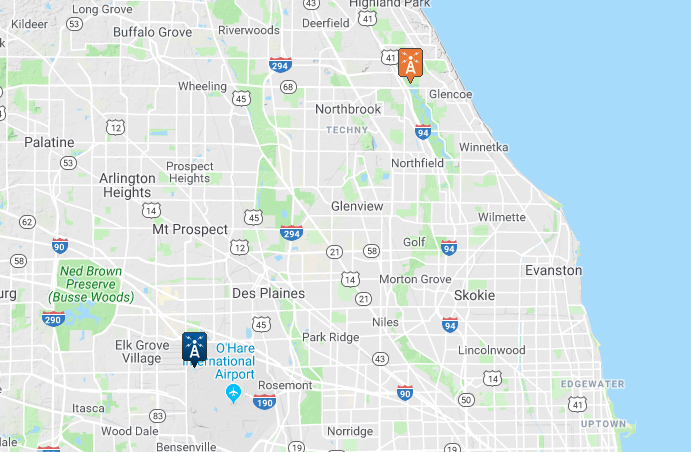
\includegraphics[width=0.8\linewidth]{./photos/garden_ohare_different_colors.png}
  \centering
  \caption{In the top right is the location of the weather tower inside of the Chicago Botanical Gardens, while the bottom left shows the location of the tower in the O'Hare Airport.}
  \label{fig:garden_ohare}
\end{figure}

\begin{enumerate}
\item[] \href{https://www.ncdc.noaa.gov/cdo-web/datasets/GHCND/stations/GHCND:USW00094846/detail}{\textbf{CHICAGO OHARE INTERNATIONAL AIRPORT, IL US}}\newline
 - Source: \href{https://www.ncdc.noaa.gov/cdo-web/search}{National Centers for Environmental Information}\newline
 - \href{https://www1.ncdc.noaa.gov/pub/data/cdo/documentation/GHCND_documentation.pdf}{GHCN (Global Historical Climatology Network) Daily Documentation}\newline
  - ID	GHCND:USW00094846  \newline
  - 41.995 N 87.9336 W \newline
 - \href{https://www.flychicago.com/ohare/home/pages/default.aspx}{Airport Information}
 
\begin{figure}[h!]
  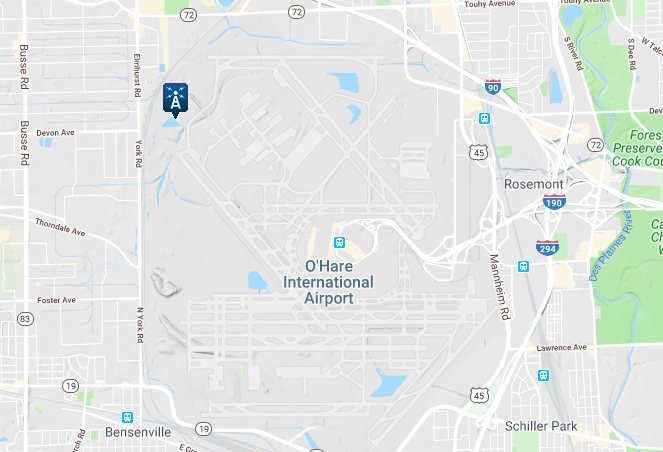
\includegraphics[width=0.5\textwidth]{./photos/ohare.png}
  \centering
  \caption{In the top left is the location of the weather tower inside of O'Hare Airport.}
  \label{fig:ohare}
\end{figure}

\item[] \href{https://www.ncdc.noaa.gov/cdo-web/datasets/GHCND/stations/GHCND:USC00111497/detail}{\textbf{CHICAGO BOTANIC GARDEN, IL US}}\newline
 - Source: \href{https://www.ncdc.noaa.gov/cdo-web/search}{National Centers for Environmental Information}\newline
 - \href{https://www1.ncdc.noaa.gov/pub/data/cdo/documentation/GHCND_documentation.pdf}{GHCN (Global Historical Climatology Network) ? Daily Documentation}\newline
  - ID GHCND:USC00111497\newline
  - 42.13987 N 87.78537 W\newline
 - \href{https://www.chicagobotanic.org/?gclid=CjwKCAjw8e7mBRBsEiwAPVxxiFAzbi0I4VKZUO1z3uxcDI36xORzYwbOtmUWGVoUqxRHEi8elJFV2RoCmaoQAvD_BwE}{Garden Information}
 
\begin{figure}[h!]
  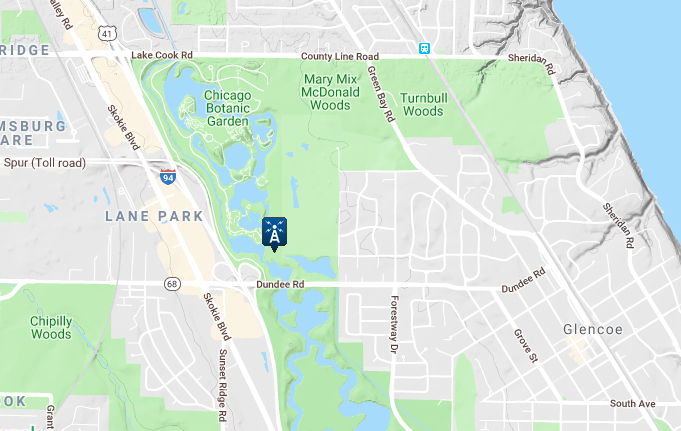
\includegraphics[width=0.5\textwidth]{./photos/garden.png}
  \centering
  \caption{The weather tower at the Chicago Botanical Gardens.}
  \label{fig:garden}
\end{figure}

 
\item[] \href{https://www.google.com/search?q=lake+michigan&oq=lake+michigan&aqs=chrome.0.69i59j69i60l3j69i59j0.3015j0j9&sourceid=chrome&ie=UTF-8}{\textbf{Lake Michigan}}
\newline
 - Source: \href{https://coastwatch.glerl.noaa.gov/statistic/statistic.html}{Great Lakes Statistics: Average Surface Water Temperature from the Great Lakes Surface Environmental Analysis (GLSEA)}\newline
 - 44.0 -87.0 (44� 00' 0.00" N 87� 00' 0.00" W)\newline
 - \href{https://coastwatch.glerl.noaa.gov/ftp/glsea/avgtemps/2018/glsea-temps2018_1024.dat}{Data Set for 2018}

\item[] \href{https://www.ndbc.noaa.gov/station_page.php?station=fsti2}{\textbf{Station FSTI2 - Foster Ave., Chicago, IL}} \newline
 - Source: \href{https://www.ndbc.noaa.gov/}{National Data Buoy Center} \newline
 - Owned and maintained by \href{https://www.ndbc.noaa.gov/ndbcexit.php?url=https://wqdatalive.com/public/16&blurb=Chicago+Park+District}{Chicago Park District}\newline
  - 41.976 N 87.648 W (41�58'35" N 87�38'51" W)
\end{enumerate}

\begin{figure}[h!]
  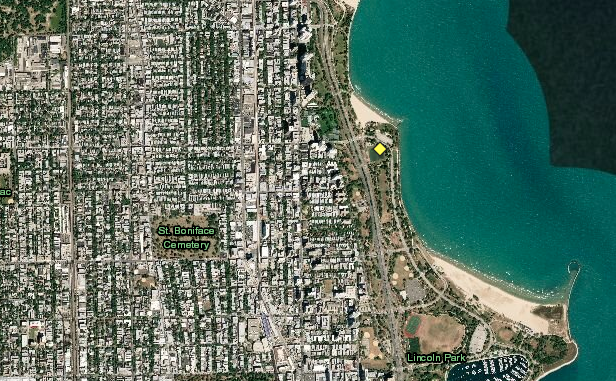
\includegraphics[width=0.5\textwidth]{./photos/FSTI2.png}
  \centering
  \caption{In the top left is the location of the weather tower inside of O'Hare Airport.}
  \label{fig:buoy}
\end{figure}


\textbf{Data}
\begin{enumerate}
\item[] \text{Links}
	\begin{enumerate}
\item[] \href{https://render.githubusercontent.com/view/ipynb?commit=3611d432f79b839ababa4ab30f3e6c71b4c65107&enc_url=68747470733a2f2f7261772e67697468756275736572636f6e74656e742e636f6d2f426c616b6557616c6c6163652f4c616b655f4d6963686967616e5f496e666c75656e6365732f333631316434333266373962383339616261626134616233306633653663373162346336353130372f646174612f446174615f44696374696f6e61726965732f446174615f44696374696f6e6172792e6970796e62&nwo=BlakeWallace%2FLake_Michigan_Influences&path=data%2FData_Dictionaries%2FData_Dictionary.ipynb&repository_id=183659877&repository_type=Repository#Data-Dictionary}{\textbf{Data Dictionary}}
\item[] \href{https://www.ndbc.noaa.gov/measdes.shtml}{\textbf{Bouy Data Dictionary}}
\item[] \href{https://www1.ncdc.noaa.gov/pub/data/ghcn/daily/readme.txt}{\textbf{O'Hare Airport Data Dictionary}}
\item[] \href{https://www1.ncdc.noaa.gov/pub/data/ghcn/daily/readme.txt}{\textbf{Botanical Garden Data Dictionary}}

\end{enumerate}

\item[] \text{"The five core values are:"}
\begin{enumerate}
 \item[] \textbf{ohare\_prcp} - Precipitation (PRCP) (inches)
 \item[] \textbf{ohare\_snfall} - Snowfall (SNOW) (inches)
 \item[] \textbf{ohare\_sndpth} - Snow depth (SNWD) (inches) 
 \item[] \textbf{ohare\_maxtmp} - Maximum temperature (TMAX) (Fahrenheit)
 \item[] \textbf{ohare\_mintmp} - Minimum temperature (TMIN) (Fahrenheit)
\end{enumerate}


\item[] \text{Other Features}
\begin{enumerate}
\item[] \textbf{lake-temp} - Average Daily Surface Water Temperature for Lake Michigan 	(Fahrenheit) 
 \item[] \textbf{garden\_prcp} - Precipitation (PRCP) (inches)
 \item[] \textbf{garden\_maxtmp} - Maximum temperature (TMAX) (Fahrenheit)
 \item[] \textbf{garden\_mintmp} - Minimum temperature (TMIN) (Fahrenheit)
 \item[] \textbf{garden\_tobs} - Temperature at time of observation (TOBS) (Fahrenheit)
 \item[] \textbf{ohare\_wspd} - Average daily wind speed (AWND) (miles per hour) 
 \item[] \textbf{ohare\_atmp} - Average Temperature (TAVG) (Fahrenheit)
 \item[] \textbf{ohare\_w2dir} - Direction of fastest 2-minute wind (WDF2) (the direction the wind is coming from in degrees clockwise from true N)  
 \item[] \textbf{ohare\_w2spd} - Fastest 2-minute wind speed (WSF2) (miles per hour)
\end{enumerate}

\item[] \text{Feature Engineering}
\begin{enumerate}
 \item[] \textbf{target} - absolute difference between the precipitation measurements at Ohare and the garden ( ohare\_prcp - garden\_prcp )
 \item[] \textbf{garden\_didrain} - categorical, 1 for yes, 0 for no
 \item[] \textbf{ohare\_didrain} - categorical, 1 for yes, 0 for no
 \item[] \textbf{garden\_medtmp} - Median daily temperature at the Garden/ midpoint between the max and min temperatures ( (garden\_maxtmp + garden\_mintmp)/2 )
 \item[] \textbf{ohare\_medtmp} - Median daily temperature at ohare/ midpoint between the max and min temperatures ( (ohare\_maxtmp + ohare\_mintmp)/2 )
 \item[] \textbf{tmpdiff} - difference between the median temperatures at ohare and the garden ( ohare\_medtmp - garden\_medtmp )
 \end{enumerate}  
 \end{enumerate}
 
  







\item \textbf{Data Cleaning/Data Manipulation/EDA}: 


Figure \ref{fig:ohare} shows the .








\item \textbf{Tests and Evaluation}:

\begin{table}[!h]
  \begin{center}
      \caption{Statistical Tests with Results}
      
	          \begin{tabular}{|c|c|c|c|c|c|}
		     \hline
			\textbf{Data}  & \textbf{t-score} & \textbf{p-value} & \textbf{Significance} & 					\textbf{Gardens Avg (F)} & \textbf{Ohare Avg (F)} \\ \hline
			All Data    & 0.5876  & 0.5568  & None         & 59.24           & 59.43         \\ 				\hline
			No Rain     & 3.285   & 0.0010  & Yes          & 58.99           & 60.57         \\ \hline
			Both Rain   & -2.629  & 0.0086  & Yes          & 59.48           & 57.7          \\ \hline
			ohareRain   & -1.9557 & 0.0506  & None         & 59.06           & 57.43         \\ 				\hline
			gardensRain & 0.0904  & 0.9280  & None         & 59.99           & 60.07         \\ 				\hline
	\end{tabular}
  \end{center}
\end{table}


\item \textbf{Models and Evaluation}:

\begin{table}[h]
  \begin{center}
    \caption{Predictive Models with their scores}
		\begin{tabular}{|c|c|c|c|c|c|}
			\hline
				\textbf{Model}   & \textbf{Training score*} & \textbf{Testing score*} & 						\textbf{Training MSE**} & \textbf{Testing MSE**} & \textbf{Cross 					Validation} \\ \hline
				Linear no poly                          & 0.0825         & 0.1052        & 0.0933       					& 0.0683      & 0.0785           \\ \hline
				Linear gs                               & 0.1222         & 0.1329        & 0.0893       & 					0.0662      & 0.0984           \\ \hline
				Decision Tree                           & 0.1139         & 0.0691        & 0.0901       					& 0.0711      & 0.0429           \\ \hline
				Decision Tree gs                        & 0.0937         & 0.0584        & 0.0922       					& 0.0719      & 0.0450           \\ \hline
				Random Forest                           & 0.8614         & 0.0517        & 0.0134       					& 0.0724      & 0.0554           \\ \hline
				Random Forest                           & 0.8711         & 0.1078        & 0.0131       					& 0.0681      & 0.0770           \\ \hline
				Random Forest gs                        & 0.8658         & 0.0905        & 0.0136       					& 0.0694      & 0.0651           \\ \hline
				Random Forest                           & 0.8677         & 0.0682        & 0.0135       					& 0.0711      & 0.0660           \\ \hline
				Random Forest                           & 0.8704         & 0.1153        & 0.0132       					& 0.0676      & 0.0767           \\ \hline
				Random Forest                           & 0.8080         & 0.0957        & 0.0195       					& 0.0690      & 0.0787           \\ \hline
				Random Forest ada                       & 0.9547         & 0.0549        & 0.0331       					& 0.0722      & 0.0331           \\ \hline
				Random Forest ada                       & 0.9445         & 0.0525        & 0.0056       					& 0.0723      & 0.0283           \\ \hline
				\multicolumn{1}{|l|}{Random Forest bag} & 0.6735         & 0.1130        & 					0.0332       & 0.0677      & 0.0928           \\ \hline
				\multicolumn{1}{|l|}{Random Forest bag} & 0.6705         & 0.1239        & 					0.0335       & 0.0669      & 0.0943           \\ \hline
		\end{tabular}
	\end{center}
\textbf{*} The score refers to the Coefficient of Determination. 

\textbf{**} MSE - Mean Squared Error

\textbf{gs} denotes a Grid Search was performed.

\textbf{ada} denotes an Ada Boost model was performed.
\end{table}

\item \textbf{Resources}:

\end{enumerate}

% --------------------------------------------------------------
%     You don't have to mess with anything below this line.
% --------------------------------------------------------------
 
\end{document}